\documentclass[11pt,a4paper]{article}
\usepackage[utf8]{inputenc}
\usepackage[a4paper,top=1in,bottom=0.6in,left=1in,right=1in]{geometry}
\usepackage{graphicx}
\usepackage{parskip}

\pagestyle{empty}

\begin{document}

\noindent
\begin{minipage}[t]{0.45\textwidth}
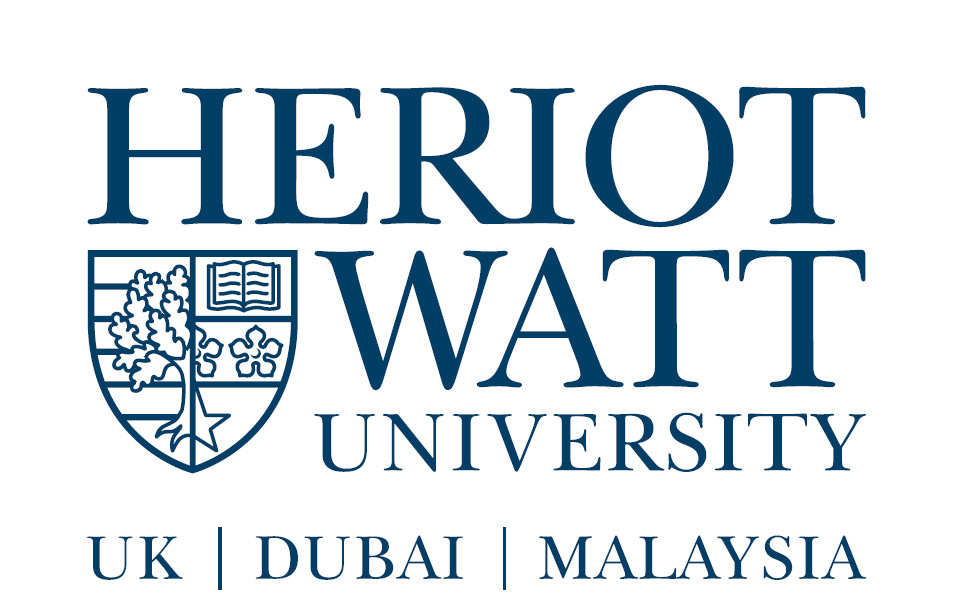
\includegraphics[width=0.52\textwidth]{figures/hwu-global-logo.jpg}
\end{minipage}%
\begin{minipage}[t]{0.55\textwidth}
\raggedleft \today
\end{minipage}

\vspace{1.0em}

Professor Lei Ya\\
Professor Vlado Vivoda\\
Editors, \textit{Resources Policy}

\vspace{0.8em}

Dear Professor Lei and Professor Vivoda,

Please find attached our Perspective manuscript, ``Beyond Critical Minerals Targets: Digital Rock Physics as Infrastructure for Secure and Circular Supply Chains'', for consideration in \textit{Resources Policy}.

The manuscript argues that UK and European critical-minerals strategies are entering an implementation phase. Policy frameworks such as the EU Critical Raw Materials Act and the UK's Vision 2035 have set ambitious goals for domestic extraction, processing, recycling, circularity, and supply-chain resilience. Achieving those goals will require more than project designation, permitting reform, and numerical targets. It will also require pre-competitive measurement, modelling, and data infrastructure capable of determining which complex ores, brines, waste streams, and recycling feedstocks can be processed viably and with lower environmental impact.

We position digital rock physics as enabling infrastructure for critical-minerals policy. By linking three-dimensional imaging, correlative chemistry, AI-enabled image analysis, and pore-scale modelling to resource-efficiency and circularity decisions, the manuscript shows how digital rock physics can support implementation across ore characterisation, liberation prediction, leaching, direct lithium extraction, mine-waste valorisation, and battery recycling. The central policy contribution is a UK-European agenda for translational demonstrators, cross-disciplinary training, a Digital Ore Passport standard, a federated Digital Ore Database, and integrated geo-reactive endstations.

We believe the manuscript is a strong fit for \textit{Resources Policy} because it addresses strategic minerals and their supply, mineral governance, sustainable resource development, circularity, and the policy design of shared research infrastructure. Its focus is not a methods review, but a resource-policy argument about how governments can move from critical-minerals targets and project lists to the practical implementation systems needed to deliver lower-impact and circular supply chains at scale.

The author team brings together expertise in digital rock physics, porous media imaging, critical-minerals policy, and energy-transition analysis: Hannah P. Menke, Heriot-Watt University; Alessio Scanziani, International Energy Agency; and Maja R\"ucker, Eindhoven University of Technology and the Max Planck Institute for Polymer Research.

This manuscript is not under consideration elsewhere.

Thank you for considering our submission.

Best wishes,

\vspace{2.7em}

Dr Hannah P. Menke\\
on behalf of all authors

\end{document}
